				%%%% patron de format latex pour rfia 2000.
				%%%% sans garanties. Plaintes \`a envoyer \`a \dev\null.
				%%%% deux colonnes pas de num\'erotation et 10 points
				%%%% necessite les fichiers a4.sty french.sty et rfia2000.sty
				
				%%%% Pour \LaTeXe
				\documentclass[a4paper,twoside,french]{article}
				\usepackage{rfia2000}
				\usepackage[T1]{fontenc}
				\usepackage[francais]{babel}
				\usepackage[utf8]{inputenc}
				\usepackage{lmodern}
				\usepackage[noend]{algpseudocode}
				\usepackage{subcaption}
				\usepackage{subfig} 
				\usepackage{usual}
				\usepackage{graphicx}
				\usepackage[rflt]{floatflt}
				\pagestyle{plain}
				
				\begin{document}
				%%%%%Pas de date
				\date{}
				%%%%% Titre gras 14 points
				\title{\Large\bf Réparation de plans dans les HTNs réactifs en utilisant la planification symbolique
				       }
			
				\author{\begin{tabular}[t]{c@{\extracolsep{6em}}c@{\extracolsep{6em}}c}
				%%%% pour quatre auteurs
				%%%%\author{\begin{tabular}[t]{c@{\extracolsep{4em}}c@{\extracolsep{4em}}c@{\extracolsep{4em}}c}
				%%%%pour plus d\'ebrouillez-vous !
				Lydia Ould Ouali${}^1$  & Charles Rich${}^2$ & Nicolas Sabouret${}^1$\\
				\end{tabular}
				{} \\
				 \\
				${}^1$        LIMSI-CNRS, UPR 3251, Orsay, France \& Univ. Paris-Sud, Orsay, France \\
				${}^2$        	Worcester Polytechnic Institute, Worcester, MA, USA\\
				%Mon adresse complète \\
				%Mon adresse électronique
				}
				\maketitle
				%%%%  Pas de num\'erotation sur la page de titre
				\thispagestyle{empty}
				\subsection*{R\'esum\'e}
				Construire des modèles formels pour planifier les prochaines actions d'un agent est un problème crucial en Intelligence Artificielle. Dans ce travail, nous proposons de combiner deux approches connues, à savoir les réseaux de tâches hiérarchiques (HTNs) et la planification symbolique linéaire. La motivation principale de cette approche hybride est de d'assurer la réparation des cassures durant l'exécution du HTN en invoquant  dynamiquement un planificateur symbolique. Ce travail nous a aussi permis de mettre en exergue  les problèmes liés à la combinaison de la modélisation procédurale et symbolique. Nous avons implémenté notre approche qui combine une HTN réactif appelé Disco et le planificateur STRIPS implémenté en Prolog, et nous avons conduit des évaluations préliminaires.
				\subsection*{Mots Clef}
				HTN réactif, planification symbolique, réparation de cassures.
				
				\subsection*{Abstract}
				Building formal models of the world and using them to plan future
				action is a central problem in artificial intelligence.  In this
				work, we combine two well-known approaches to this problem, namely,
				reactive hierarchical task networks (HTNs) and symbolic linear
				planning.  The practical motivation for this hybrid approach was to
				recover from breakdowns in HTN execution by dynamically invoking
				symbolic planning.  This work also reflects, however, on the deeper
				issue of tradeoffs between procedural and symbolic modeling.  We
				have implemented our approach in a system that combines a reactive
				HTN engine, called Disco, with a STRIPS planner implemented in
				Prolog, and conducted a preliminary evaluation.
				\subsection*{Keywords}
				Reactive HTN, symbolic linear planning, breakdowns, recovery.
				
				
		\section{Introduction}
		Les r\'eseaux de t\^aches hi\'erarchiques ou HTN \cite{erol1994htn} (Hierarchical task networks) sont largement utilis\'es pour contr\^oler des agents et des robots \'evoluant dans des environnements dynamiques. Il existe dans la litt\'erature diff\'erentes formalisations et repr\'esentations graphiques. Nous utiliserons ici une simple repr\'esentation en arbre, avec  différents niveaux de  n\oe uds {\em tâches}  et des  n\oe uds de {\em décompositions}. Un HTN est donc défini avec un n\oe ud tâche au niveau de la racine. Les feuilles constituent des {\em tâches primitives}, correspondant aux actions de l'agent dans le monde. Les autres n\oe uds de l'arbre définissent soit des {\em tâches abstraites} à décomposer (c'est par exemple le cas de la racine de l'arbre), soit des \emph{recettes} décrivant une décomposition possible en sous-tâches (elles-mêmes décomposables à leur tour, jusqu'à atteindre des tâches primitives).

		\par Ces HTNs sont g\'en\'eralement cod\'es \`a la main par un modélisateur qui définit la décomposition des tâches en recettes et en sous-tâches (éventuellement partiellement ordonn\'ees). En plus de cette d\'ecomposition, la plupart des HTNs sont d\'efinis avec des conditions pour le contrôle de l'exécution. Ainsi, le modélisateur peut définir pour chaque recette des \emph{conditions d'applicabilité} qui déterminent l'applicabilité de la recette dans l'état courant, et pour chaque tâche des pr\'econditions et des post-conditions. Une tâche ne peut être effectuée que si ses préconditions sont valides et une tâche est considérée comme réussie si ses post-conditions sont satisfaites.
						
		\par \`A l'origine, les HTN sont une extension hi\'erarchique des plans lin\'eaires classiques (e.g. STRIPS \cite{fikes1972strips}), et comme pour les modèles classiques, les conditions associ\'ees aux t\^aches sont dites \textit{symboliques}, \emph{i.e.} elles sont \'ecrites en logique formelle qui permet à un moteur d'inf\'erence de raisonner dessus. La principale difficulté, comme l'a souligné \cite{gil1992acquiring}, réside dans la modélisation complète et fidèle d'une monde complexe à l'aide de prédicats. En r\'eponse à ces difficult\'es li\'ees \`a la mod\`elisation des connaissances symboliques, une variante appel\'ee HTNs \textit{réactifs} a \'et\'e developp\'ee dans laquelle les conditions sont \textit{proc\'edurales}, \emph{i.e.} elles sont \'ecrites dans un langage de programmation et \'evalu\'ee par un interpr\'eteur de ce langage de programmation. Les HTNs réactifs sont utilis\'es par exemple dans le domaine des jeux vid\'eos sous le nom de \emph{behaviour tree}\footnote{See http://aigamedev.com/open/article/popular-behavior-tree-design}.	
		\par Notre travail porte sur les HTNs réactifs et, en particulier, sur la réparation des cassures (ou \emph{breakdowns}) qui peuvent survenir durant l'exécution. L'idée principale est d'ajouter une petite proportion de conditions symboliques au HTN réactif afin de permettre à un planificateur linéaire de produire des plans de réparation locaux.
				\begin{figure}[t]
					\centerline{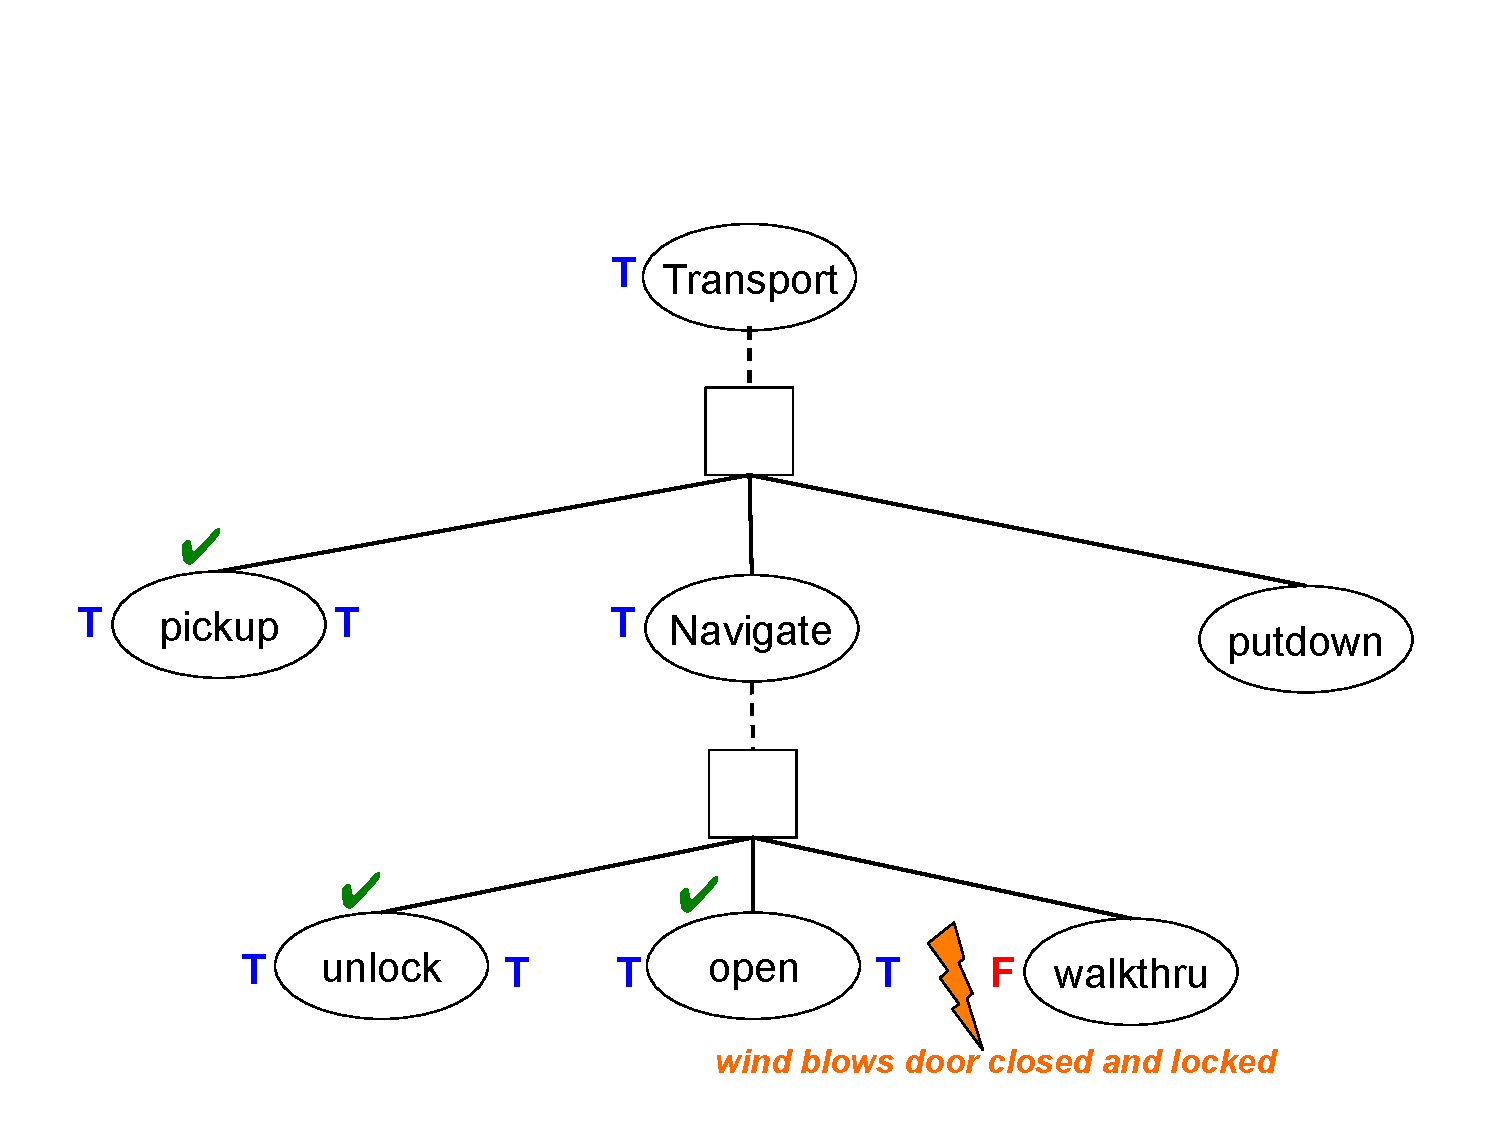
\includegraphics[width=3in]{figs/wind}}
					\vskip 8pt
					\defig{wind}{Cassure dans l'exécution du HTN après que le vent a fait claquer la porte et l'a bloquée. Les coches indiquent les tâches dont l'exécution est terminée. ``T'' représente une condition dont l'évaluation a retourné \emph{vrai}; ``F'' représente une condition qui a retourné \emph{faux}.}
				\end{figure}

		\section{Motivations}
		\label{sec:motivation}
		Afin de mieux introduire et expliquer notre travail, considérons un exemple simple mais intuitif d'une cassure dans l'exécution d'un HTN et sa réparation, illustré dans la  \fig{wind}. Il s'agit d'implémenter en HTN le comportement d'un robot pour transporter un objet a travers une porte fermée. Dans le HTN, la tâche but {\em transport}, est décomposée en trois étapes: ramasser l'objet ({\em pickup}), manipuler la porte {\em(navigate)} et poser l'object {\em(putdown)}. La tâche {\em navigate} est à son tour décomposée en quatre étapes: déverrouiller  la porte {\em(unlock)}, l'ouvrir {\em(open)} et franchir la porte {\em(walkthrough)}. Chacune de ces tâches est représentée par un ovale dans la \fig{wind}. Les boîtes représentent les différentes alternatives de décomposition qui peuvent être ignorées dans cet exemple. Au moment de l'exécution décrit dans la \fig{wind}, le robot a ramassé l'objet, déverrouillé et ouvert la porte avec succès. Cependant, avant que la précondition de la tâche {\em walkthrough} ne soit évaluée, le vent souffle et la porte de ferme et se verrouille (l'exemple ne vise pas à être réaliste mais à illustrer notre propos). La précondition de la tâche {\em walkthrough} évalue si la porte est ouverte et retourne faux. À ce moment, aucune tâche ne peut être exécutée dans le HTN et c'est ce que nous appelons une {\em cassure}. Il n'est pas rare qu'un HTN réactif rencontre des cassures, spécialement dans le cas d'exécution dans des environnements dynamiques et complexes. Cependant, en analysant la cassure produite dans cet exemple, la solution montrée dans la \fig{recover} parait évidente: déverrouiller la porte et l'ouvrir. Trouver une solution pour cette cassure est un problème trivial pour un planificateur linéaire symbolique comme STRIPS si les (pré/post)-conditions des tâches primitives correspondantes étaient spécifiées symboliquement.
					\begin{figure}[t]
						\centerline{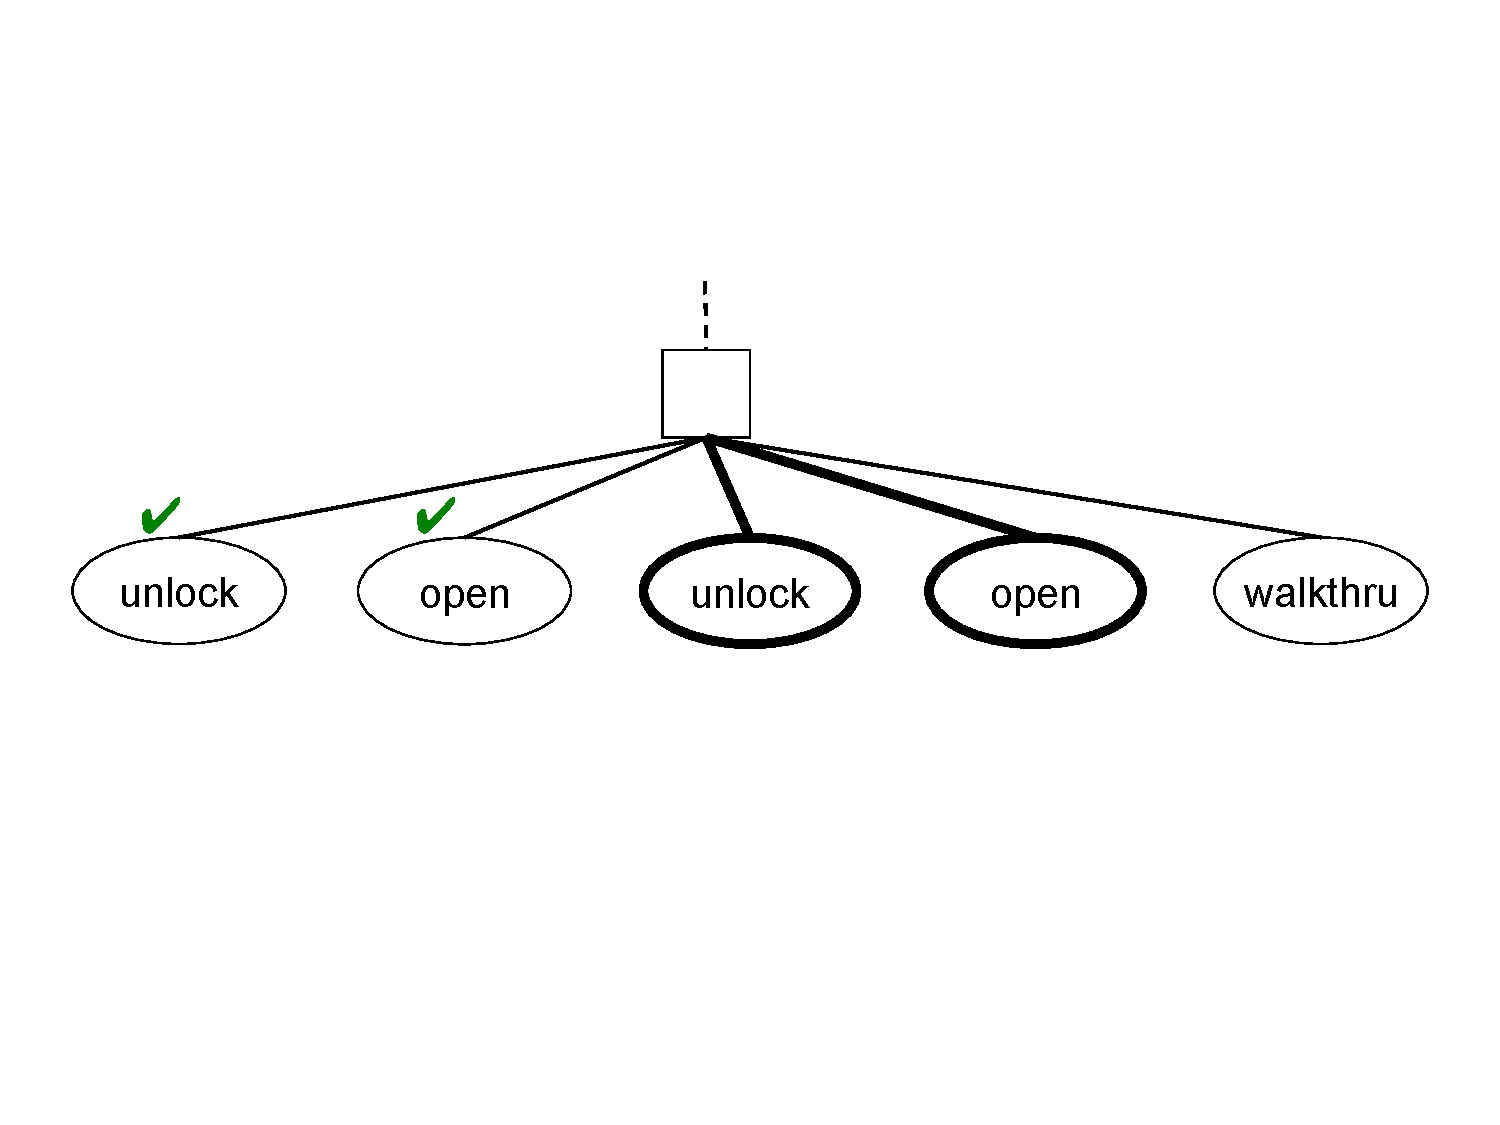
\includegraphics[width=3in]{figs/recover}}
						\vskip 8pt
						\defig{recover}{Séquence de deux tâches primitives (en gras) ajoutées au plan hiérarchique de la tâche ``navigate'' pour réparer la cassure de la \fig{wind}.}
					\end{figure}
		
	
		\par Or justement, ce qui caractérise un HTN réactif, c'est que \emph{les pré et post-conditions sont définies à l'aide de scripts} (elles sont définies en langage procédural et évaluées par un interpréteur approprié à ce langage) et \emph{ne peuvent donc pas être manipulés comme des connaissances symboliques}. La \fig{procedures} montre les  conditions procédurales définies dans le plan {\em Navigate} comme elles seraient typiquement écrites par exemple en JavaScript. Par exemple, la procédure ``isOpen()'' appelle un code spécifique dans le système de capteurs du robot pour évaluer si la porte est actuellement ouverte. À titre de comparaison, la \fig{features} montre la formalisation des mêmes tâches en STRIPS. 
		
		\par Supposons que lorsque la cassure a été détectée dans l'exemple de la \fig{wind}, le moteur d'exécution du HTN contenait la connaissance symbolique qui est fournie sur la \fig{features}. La réparation de la cassure pourrait donc être traitée comme une problème de planification STRIPS (voir \fig{planning}) dans lequel l'état initial est représenté par l'état courant du monde et l'état final est la précondition échouée de la tâche {\em walkthrough} (la porte est ouverte). Un simple chainage arrière peut rapidement trouver une séquence d'actions (à savoir déverrouiller et ouvrir la porte). Le plan produit est ensuite intégré au HTN comme dans la \fig{recover} afin de permettre au HTN de reprendre son exécution.  Le but de cet article est de généraliser la solution de cet exemple en algorithme de réparation de cassures qui soit indépendant des applications et auquel on associe une méthodologie de modélisation des HTNs réactifs.
		
			\begin{figure}[t]
				\centering
				\begin{subfigure}{2.3in}
					\centerline{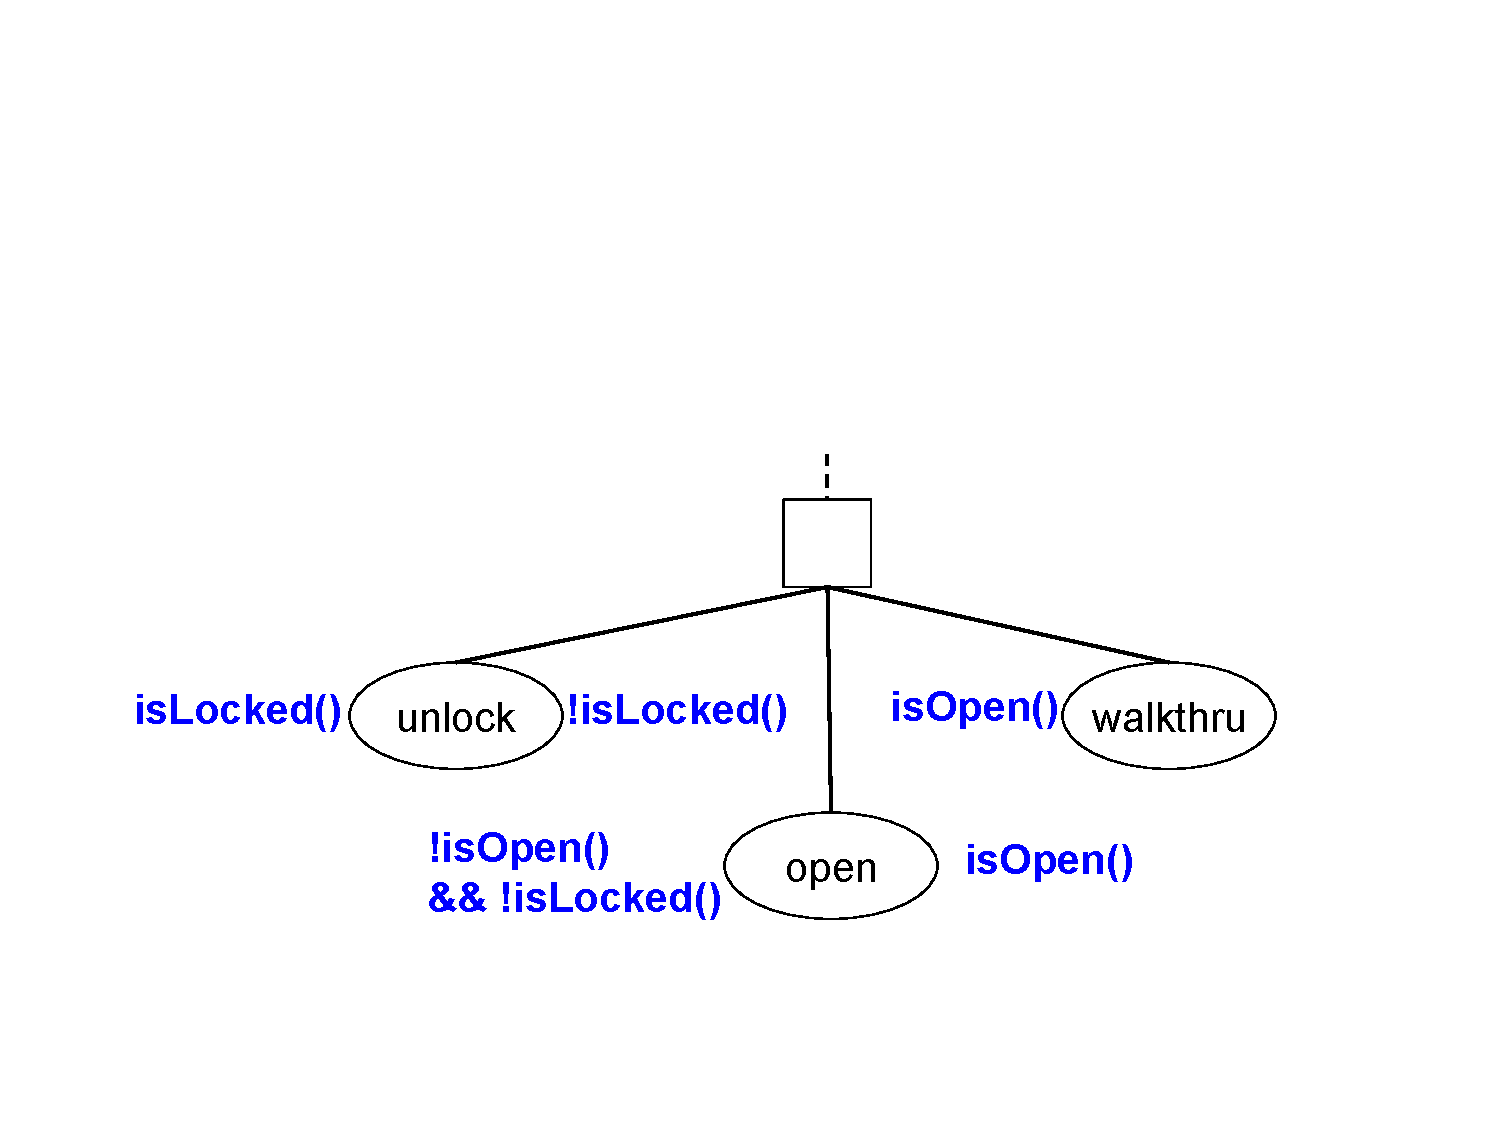
\includegraphics[width=2.4in]{figs/procedures}}
					\vskip 8pt 
					\defig{procedures}{Conditions procédurales }
				\end{subfigure}
				\hfill
				\begin{subfigure}{2.3in}
					\centerline{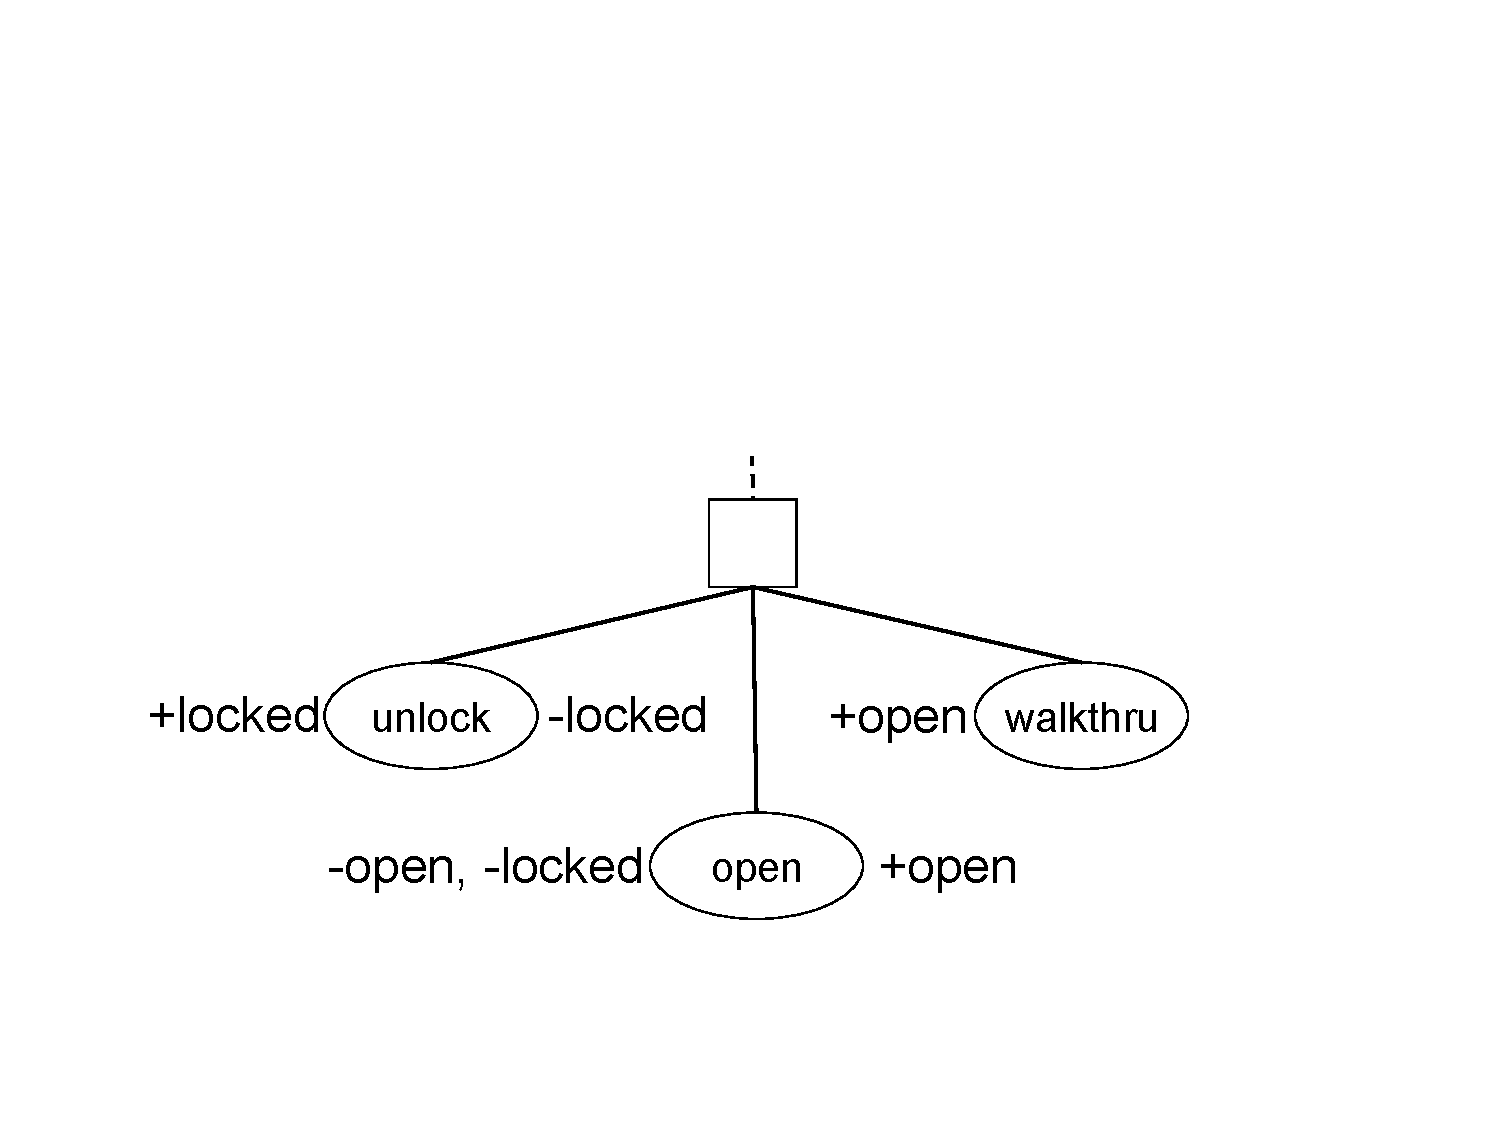
\includegraphics[width=2.4in]{figs/features}}
					\vskip 8pt 
					\defig{features}{Représentation symbolique des conditions}
				\end{subfigure}
				\vskip 8pt
				\defig{comparison}{Conditions procédurales versus symboliques pour le plan Navigate.}
			\end{figure}
	
		\begin{figure}[]
			\centerline{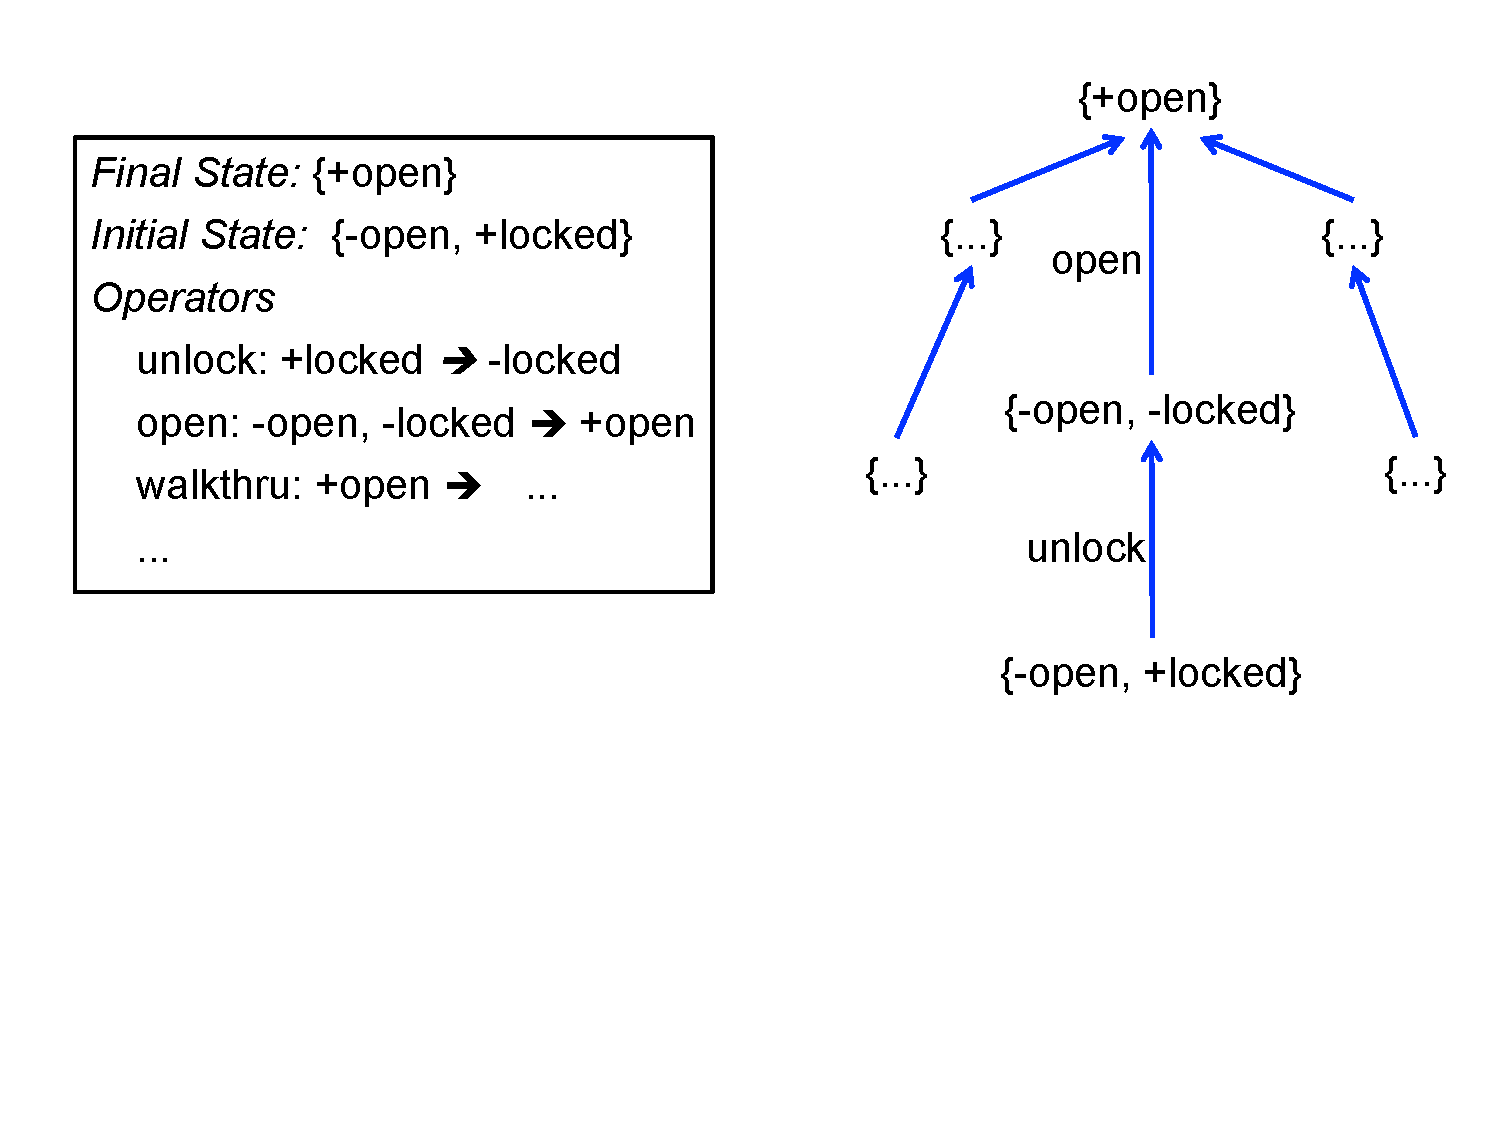
\includegraphics[width=3.7in, height=1in]{figs/planning}}
			\vskip 8pt
			\defig{planning}{Réparation de la cassure de la \fig{wind} comme un problème de planification STRIPS.}
		\end{figure}
		 
		
		\section {Travaux connexes}
		La question que pourrait soulever la section précédente est pourquoi ne pas utiliser seulement la planification symbolique au lieu d'un HTN réactif et appliquer les solutions existantes de réparation des cassures? a problématique de la réparation des cassures durant l'exécution a déjà été étudiée dans le domaine des HTNs symboliques et de nombreux modèles ont été proposés\cite{boella2002replanning,van2005plan,ayan2007hotride,warfield2007adaptation}. Ces techniques de réparation de plans sont généralement très efficaces.

		\par La réponse à cette question réside dans le rapport entre la modélisation du problème et l'exécution du plan produit. En effet, les planificateurs symboliques basées sur des connaissances symboliques linéaires (en langage STRIPS ou PDDL \cite{ghallab1998pddl}) ou hiérarchiques (à l'aide de HTNs) requièrent une description {\em complète} et {\em correcte} de toutes les tâches dans le domaine du problème. Si la description symbolique est incomplète ou incorrecte, les plans générés vont subir des cassures à l'exécution.

		\par Malheureusement, la recherche en IA \cite{gil1992acquiring} a montré que la modélisation d'une description logique du monde réel qui soit complète et correcte peut se révéler extrêmement difficile voir impossible en pratique. C'est pour cela que les HTNs réactifs ont été inventés: la connaissance est insérée dans les HTNs réactifs principalement à deux endroits: dans la structure de décomposition de l'arbre et dans le code pour définir les conditions procédurales (en particulier dans les conditions d'applicabilité pour les choix de décompositions). L'intérêt des HTNs réactifs provient de la facilité de modélisation sur des problèmes dont le domaine de connaissance est complexe pour être modélisé de manière symbolique. De plus, les conditions procédurales ne sont évaluées que dans l'état {\em courant} du monde (alors que les descriptions symboliques doivent être vrais dans tous les mondes possibles). Ceci n'empêche pas les HTNs réactifs de rencontrer des cassures, comme dans notre exemple, et c'est ce qui nous a conduit à proposer une approche hybride dans laquelle un HTN réactif est augmenté avec de la connaissance symbolique afin d'aider à la réparation des cassures.
		
		\par D'autre travaux avant nous ont proposé d'ajouter un module de raisonnement symbolique pour étendre les HTNs réactifs. Par exemple, Firby \cite{firby1987investigation} propose d'ordonner les tâches dans la file d'exécution du HTN et de choisir d'autres alternatives de décompositions ce qui permet au HTN de détecter les situations problématiques avant qu'elles ne se produisent. Brom \cite{brom2005hierarchical} propose d'utiliser la planification afin d'assurer l'exécution des tâches avec des contraintes de temps. Cependant, aucune de ces deux approches ne propose d'étudier la possibilité de réparer des HTN réactifs à l'aide de planification symbolique. Notre originalité est de proposer un algorithme hybride combinant le procédural et le symbolique.

		\section{L'approche hybride}
		Dans cette section, nous proposons une généralisation sur deux niveaux de l'exemple de la section 2 en considérant: (1) les différents types de cassures, (2) l'ensemble des états finaux possibles. Nous présenterons d'abord l'algorithme général de réparation de cassures et discuterons ensuite la méthodologie de modélisation associée.
			\begin{figure*}[t]
				\centering
				\begin{subfigure}{2.1in}
					\centerline{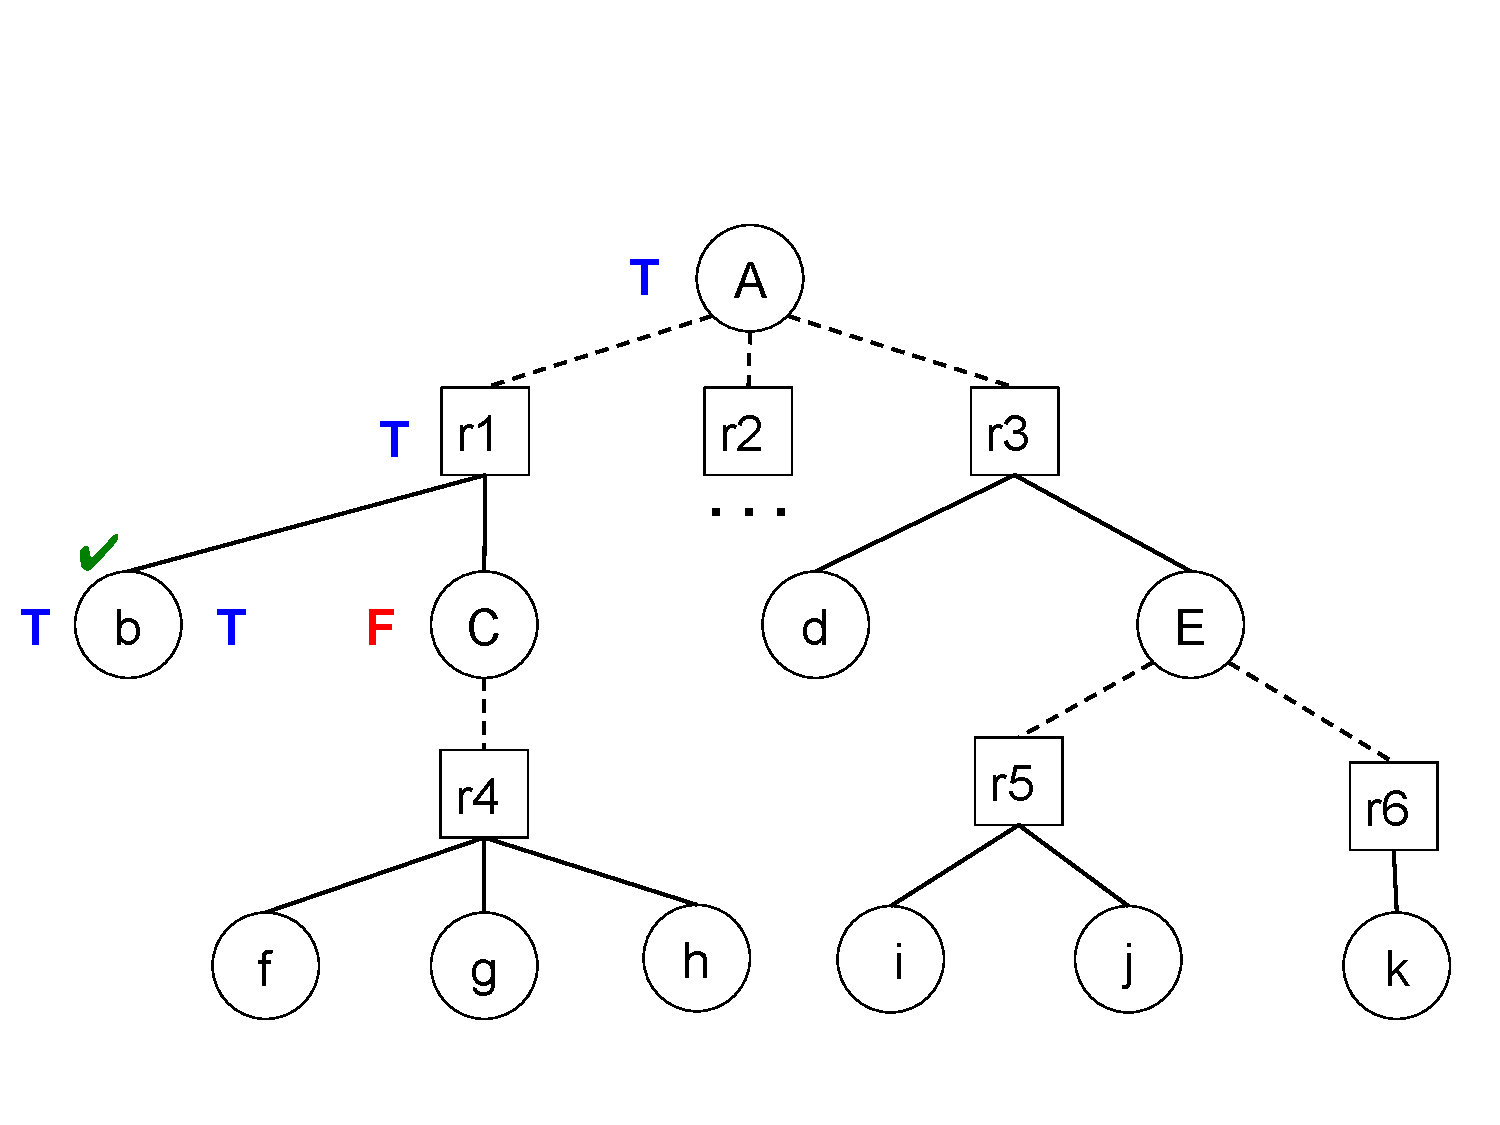
\includegraphics[height=1.3in]{figs/precondition}}
					\vskip 8pt 
					\defig{precondition}{Précondition échouée}
				\end{subfigure}
				\hfill
				\begin{subfigure}{1.4in}
					\centerline{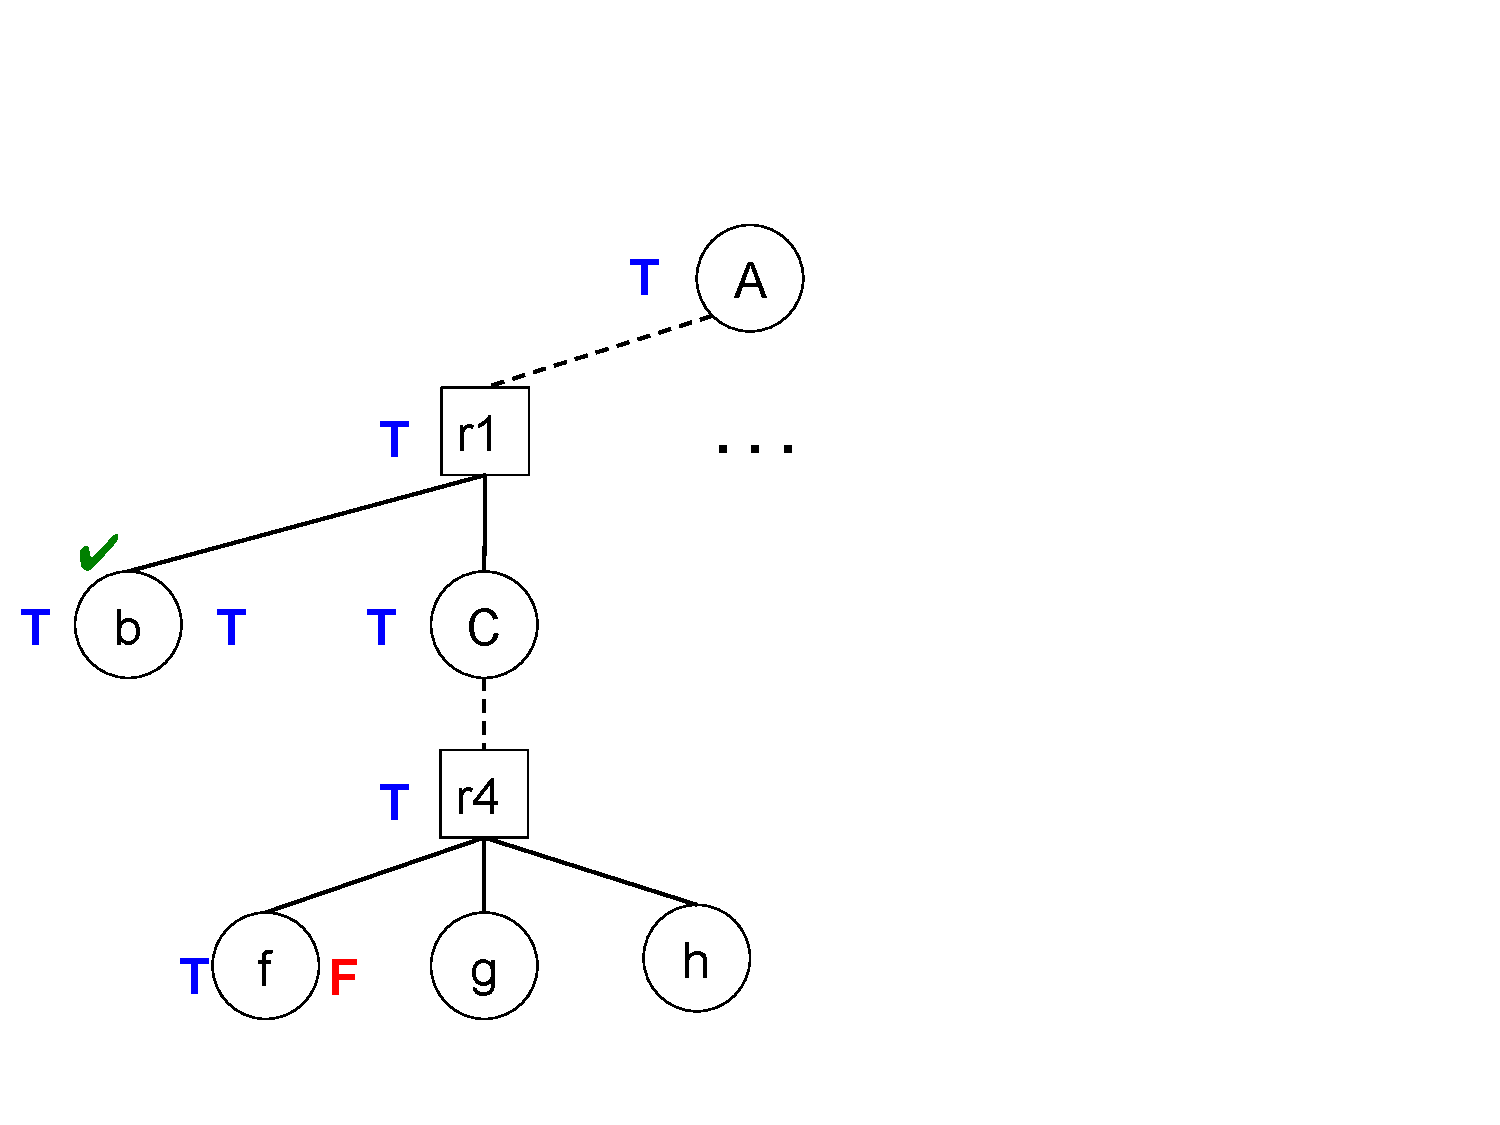
\includegraphics[height=1.3in]{figs/postcondition}}
					\vskip 8pt 
					\defig{post-condition}{post-condition échouée}
				\end{subfigure}
				\hfill
				\begin{subfigure}{1in}
					\centerline{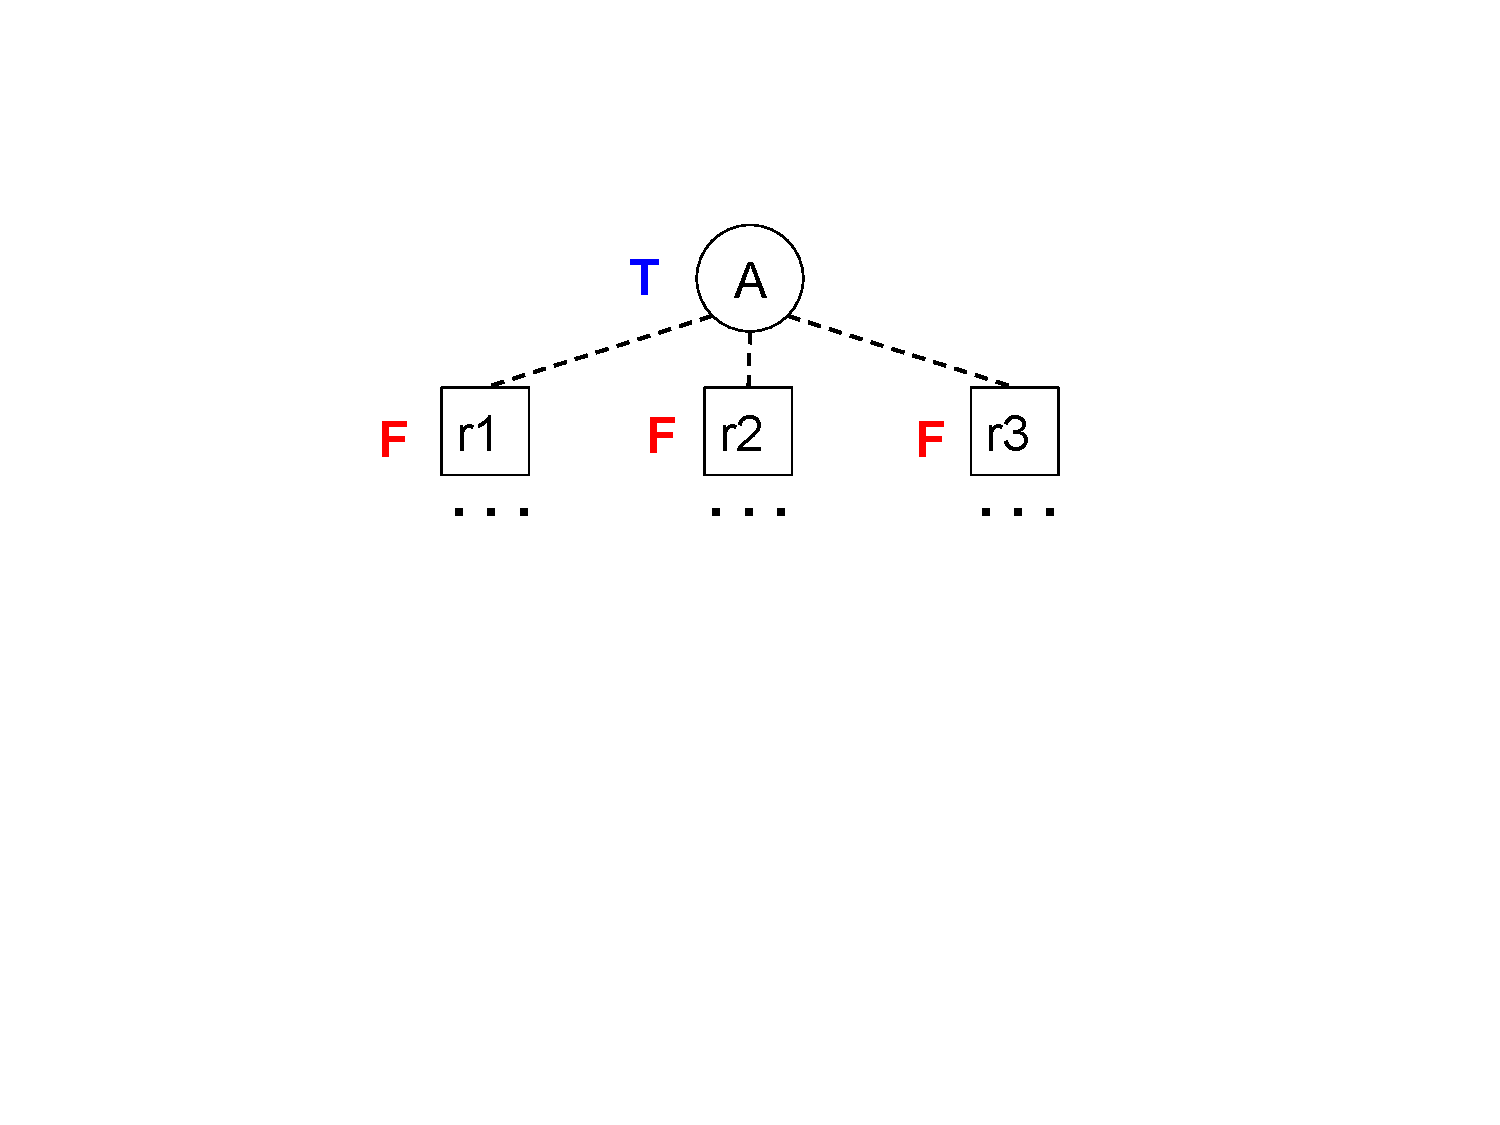
\includegraphics[height=1.3in]{figs/applicability}}
					\vskip -2pt
					\defig{applicability}{Condition d'applicabilité échouée}
				\end{subfigure}
				\vskip 4pt 
				\defig{breakdowns}{Exemples des trois types de cassures dans l'exécution d'un HTN.} 
			\end{figure*}
			
		\subsection{Les HTNs réactifs}
		\par Les HTNs réactifs peuvent être représentés comme un arbre et/ou, où les tâches sont des "et", et les n\oe uds de décomposition sont des "ou". Contrairement aux HTNs symboliques, les HTNs réactifs ne visent pas à anticiper le futur et construire un plan complet afin de l'exécuter par la suite. Ils se content seulement de calculer la prochaine tâche a exécuter à partir de l'état courant du monde. L'exécution est en profondeur d'abord, avec un parcours de gauche à droite à partir du n\oe uds racine, durant lequel les conditions sont évaluées, comme décrit ci-après. 
		\par Si l'exécution du n\oe ud courant est une tâche alors ses éventuelles préconditions représentés en procédures booléennes sont évaluées. Si elles retournent faux, alors l'exécution est interrompue \textit{(cassure)}; sinon l'exécution continue. Si la tâche est primitive, elle est directement exécutée pour changer l'état du monde. Sinon, si elle est abstraite alors les conditions d'applicabilités des n\oe uds fils (décompositions) sont évalués dans l'ordre jusqu'à l'obtention d'un n\oe ud qui retourne vrai. L'exécution continue alors avec cette décomposition. Si toutes les conditions d'applicabilités sont fausses alors  l'exécution est arrêtée \textit{(cassure)}. Une fois l'exécution de la tâche terminée, ses éventuelles post-conditions sont évaluées, si elles retournent faux, alors l'exécution est interrompue \textit{(cassure)}. Sinon l'exécution continue. Si le n\oe ud courant est un n\oe ud de décomposition, alors les n\oe uds fils (tâches) sont exécutées dans l'ordre. 
		\par La \fig{breakdowns} résume les trois types de cassures qu'un HTN peut rencontrer durant son exécution. La cassure dans l'exemple de la section 2 est causé par une précondition échouée. Cependant, cette taxonomie n'est pas apte à distinguer les raisons sous-jacentes qui peuvent provoquer des cassures. En effet, une cassure peut être causée par un changement inattendu dans le monde (\emph{e.g.} le vent dans la section 2) ou à cause d'une erreur de programmation (condition mal codée, structure d'arbre erronée). L'impossibilité de détecter les causes des cassures est une limitation intrinsèque des HTN réactifs.

		\subsection{Algorithme de réparation de plans}
		\noindent  La généralisation la plus significative de l'algorithme sur l'exemple de la section \ref{sec:motivation}, concerne le choix de l'état final pour le planificateur linéaire.  En effet, pour que l'algorithme de réparation fonctionne il a besoin d'avoir en entrée un état but à atteindre. Cependant, pour ce même exemple, différents état buts peuvent être trouvés. Par exemple, supposons que {\em walkthrough} ait une post-condition qui spécifie que le robot est dans la pièce de l'autre côté de la porte. Après la cassure, le robot peut trouver une autre méthode de réparation: trouver un plan pour satisfaire cette post-condition (par exemple, sortir de la pièce actuelle par une autre porte...). Cette procédure consiste à définir la post-condition comme un  {\em état but}  candidat pour la réparation. De la même façon, supposons que {\em walkthrough} n'a pas de représentation symbolique pour sa post-condition, mais que la post-condition symbolique de {\em navigate} spécifie l'emplacement but du robot. Dans ce cas la post-condition de {\em navigate} est considérée comme un état but de réparation. De manière similaire, si on suppose que la cassure dans notre exemple a été provoquée par l'échec de la post-condition de {\em unlock}, la représentation symbolique de la précondition de {\em walkthrough} ainsi que celles des post-conditions de {\em walkthrough} et de {\em navigate} sont de bons candidats pour la réparation.
		\par Sur la base de ce raisonnement, l'algorithme que nous présentons ci-dessous repose sur l'idée de construire les états but candidats pour la procédure de réparation à partir de l'ensemble  des conditions du HTN  affectées par la cassures (dont l'évaluation retourne faux) et qui n'ont pas encore été validées durant l'exécution. Nous pensons que cette première approximation est trop grossière (trop de candidats sont considérés) mais nous avons besoin d'étudier notre approche sur des exemples plus concrêts pour concevoir une meilleure heuristique de recherche. Il est a noter qu'une condition d'applicabilité est considérée comme candidat dans l'unique cas où toutes ses s\oe urs dans l'arbre ont été évaluées comme fausses.

		\par La \fig{pseudo} présente le pseudo-code du système hybride ainsi conçu. La procédure principale, {\sc Execute}, execute un HTN jusqu'à ce qu'il se termine (succès) ou jusqu'à ce qu'une cassure soit détectée. Le code de réparation des cassures commence à la ligne 5. La sous procédure, {\sc FindCandidates} va récursivement parcourir le HTN afin de calculer les candidats cibles pour la procédure de réparation. La procédure {\sc SymbolicPlanner} n'est pas décrite car n'importe quel planificateur linéaire peut être utilisé. De plus, comme l'ensemble des opérateurs symboliques ne change pas durant l'exécution, il n'est pas défini comme un argument explicite du planificateur symbolique. On peut voir à ligne 6 que notre approche requiert une méthode pour calculer, à partir de l'état courant, l'état initial du planificateur symbolique dans un formalisme symbolique que le planificateur puisse exploiter. Par exemple, pour l'exemple de la section 2, chaque fonction symbolique comme ``open'' doit être associée à une procédure comme ``isOpen()'' donnant sa valeur dans l'état courant. C'est là que réside la difficulté de la modélisation hybride (discutée dans la section 4.3). La ligne 8 montre que les candidats sont triés par rapport à leurs distance du n\oe ud courant dans l'arbre, en utilisant une simple métrique (par exemple le plus court chemin dans un arbre non-orienté). Notre but est ainsi de favoriser des réparations locales qui préservent au maximum la structure originale du HTN. Cependant, nous n'avons pas encore testé les performances de cette heuristique. Enfin, à la ligne 12 de la procédure {\sc execute}, quand un plan est trouvé, il doit être intégré dans le HTN pour être exécuté. Une fois le plan de réparation exécuté, le HTN récupéré la tâche de la condition réparée pour poursuivre son l'exécution. Dans l'exemple de la figure \fig{planning} la condition réparée est ``isOpen()''. Par conséquent, la prochaine tâche à exécuter après le plan de réparation est la tâche où la condition est utilisée, à savoir {\em walkthrough}.  
		\begin{figure}[t]
		
			\begin{algorithmic}[1]\small
				
				\Procedure{Execute}{$htn$}
				\While{$htn$ is not completed} 
				\State $current\gets$ next executable node in $htn$
				\If{$current\neq null$} execute $current$
				\Else\hskip 0.1in [breakdown occurred]
				\State $initial\gets$ symbolic description of current world state
				\State $candidates\gets FindCandidates(htn)$
				\State sort $candidates$ by distance from $current$
				\For{$final \in candidates$}
				\State plan$\gets$ SymbolicPlanner(initial,final)
				\If{$plan\neq null$}
				\State splice $plan$ into $htn$ between $current$ and $final$
				\State \textbf{continue} while loop above
				\EndIf
				\EndFor
				\State Recovery failed!
				\EndIf
				\EndWhile
				\EndProcedure
				\Statex
				\Procedure{FindCandidates}{$task$}
				\State $conditions\gets\emptyset$
				\State $pre\gets$ symbolic precondition of $task$
				\If{$pre\neq null\;\wedge$ procedural prec of $task$ has not evaluated to true}
				\State add $pre$ to $conditions$\EndIf
				\State $post\gets$ symbolic post-condition of $task$
				\If{$post\neq null\;\wedge$ procedural postc of $task$ has not evaluated to true}
				\State add $post$ to $conditions$
				\EndIf
				\State $applicables\gets\emptyset$
				\State $allFalse\gets true$
				\For{$decomp \in$ children of $task$}
				\For{$task\in$ children of $decomp$} $FindCandidates(task)$
				\EndFor 
				\If{$allFalse$}
				\If{procedural appl condition of $decomp$ has evaluated to false}
				\State $app\gets$ symbolic applicability condition of $decomp$
				\If{$app\neq null$} add $app$ to $applicables$\EndIf
				\Else $\;allFalse\gets$ false
				\EndIf 
				\EndIf
				\EndFor
				\If{$allFalse$} add $applicables$ to $conditions$
				\EndIf
				\State\Return $conditions$
				\EndProcedure 
				
			\end{algorithmic}
			\vskip 8pt
			\defig{pseudo}{Pseudocode de l'exécution et réparation du système HTN réactif hybride}
		\end{figure} 
		\subsection{Méthodologie de modélisation}
		Le système hybride prend avantage de la connaissance symbolique construite par l'auteur du HTN, sachant que toute condition  dans le HTN peut, ou non, avoir une représentation symbolique. Comme  nous l'avons annoncé précédemment, la difficulté liée à la réalisation d'une modélisation symbolique a conduit les auteurs des HTNs à utiliser la modélisation procédurale. Il existe donc deux problèmes méthodologiques liées à la conception d'un HTN hybride. D'une part, il faut déterminer où il est préférable d'investir l'effort nécessaire de modélisation symbolique. D'une autre part, il faut définir une stratégie qui facilite à l'auteur le processus de mixage entre le procédural et le symbolique. Notre intuition première est qu'il faut réduire la modélisation symbolique aux tâches primitives, car nous espérons que l'utilisation d'une stratégie locale pour la réparation des cassures sera plus efficace. Le choix des opérateurs à introduire au planificateur linéaire a une implication directe sur ses performances. En effet, seules les tâches primitives disposant d'une représentation symbolique de ses pré et post-conditions peuvent être incluses dans l'ensemble des opérateurs. Cependant, si une tâche abstraite dispose de ces caractéristiques, elle peut alors être  utilisée pour la réparation des cassures, en utilisant durant son exécution une de ses décompositions valables dans l'état courant. 
		\par Nous envisageons de développer un outil qui aiderait à simplifier la modélisation hybride en détectant les liens entre les deux modélisations comme dans la \fig{procedures} et générer automatiquement la représentation symbolique comme dans la \fig{features}. L'outil pourrait aussi garder l'historique des cassures et les utiliser pour guider l'auteur dans l'ajout de connaissances symboliques dans le HTN.
		
		\section{Implémentation et évaluation}
		Nous avons implémenté notre système hybride en Java en utilisant le standard ANSI/CEA-2012 \cite{rich2009building} pour la modélisation du HTN et Disco \cite{rich2012using} comme le moteur d'exécution de ce HTN. Concernant le planificateur symbolique, nous avons utilisé une simple implémentation de STRIPS  exécutée dans un environnement Java de Prolog \footnote{See http://tuprolog.apice.unibo.it}. L'utilisation de Prolog facilite l'ajout de règles de raisonnement symboliques durant le processus de planification. 
		\par Une véritable évaluation de notre approche consisterait à faire évoluer plusieurs agents dans des environnements dynamiques du monde réel et évaluer leurs performances ainsi que leur robustesse face aux cassures. En attendant, nous avons validé notre système avec une expérimentation préliminaire sur des HTNs générés synthétiquement en variant le niveau de connaissance symbolique. Nous sommes partis d'une théorie simple qui préconise que plus il y'a des connaissances symboliques dans le HTN, meilleures seront ses performances pour la réparation des cassures.
		\par La \fig{results} montre les résultats obtenus qui confirment notre hypothèse. Nos HTN synthétiques sont caractérisés par trois dimensions $R \times S \times D$, où R est le facteur de ramification d'une décomposition (recipe), S le facteur de ramification d'une tâche, D étant la profondeur du HTN. Nous avons testé deux configurations de HTNs de dimensions respectivement $3\times 3\times 3$ et $1\times 5\times 4$. Pour chaque test, nous avons aléatoirement extrait des combinaisons possibles de connaissance symbolique sur trois différent niveaux; 25\% , 50\%, 75\% (le pourcentage des conditions qui ont une représentation symbolique). Nous nous sommes restreints à ces modélisations pour des questions de temps d'exécution. La \fig{recovery} montre l'évolution des performances de réparation des cassures en fonction de l'augmentation du niveaux de connaissance symbolique. Dans la \fig{candidates}, nous nous sommes intéressés à la proportion des problèmes de planification soumis au planificateur (buts candidats) qui ont été correctement résolus. Nous pouvons remarquer que cette dernière augmente aussi en fonction du niveaux de connaissance symbolique (pour ces tests, nous avons modifié notre système pour qu'il génère un plan pour tous les candidats).
		\begin{figure}[t]
			\centering
			\begin{subfigure}{2.3in}
				\centerline{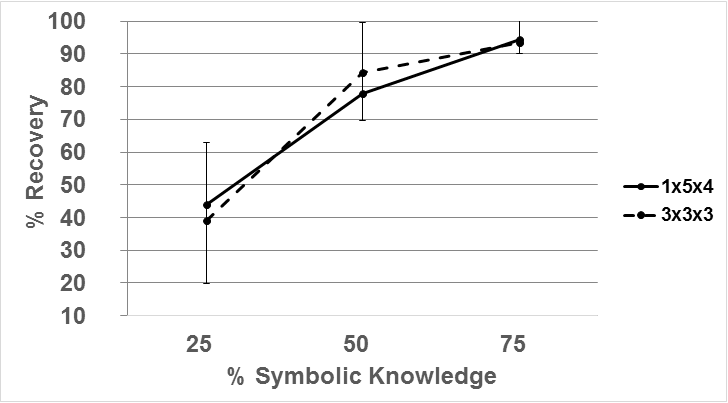
\includegraphics[width=2.3in]{figs/recovery}}
				\vskip 8pt 
				\defig{recovery}{Ration des réparation/cassure}
			\end{subfigure}
			\hfill
			\begin{subfigure}{2.3in}
				\centerline{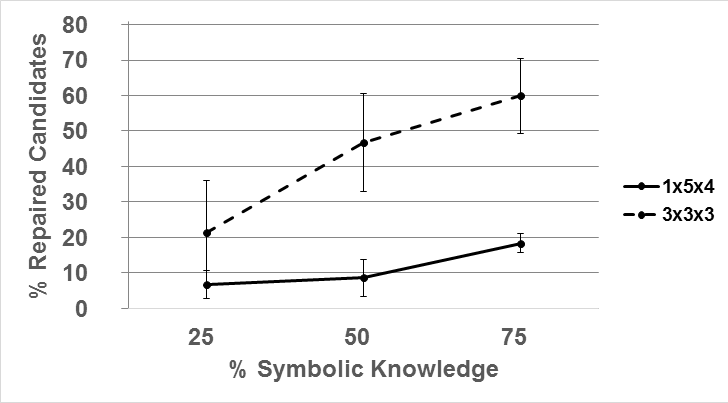
\includegraphics[width=2.3in]{figs/candidates}}
				\vskip 8pt 
				\defig{candidates}{Proportion des candidats réparés}
			\end{subfigure}
			\vskip 6pt
			\defig{results}{Résultats des expérimentations sur des HTNs générés synthétiquement avec différents niveaux de connaissances symbolique.}
		\end{figure}
\section{Conclusion}
Nous avons présenté dans cet article une première contribution pour la réparation des cassure qui consiste à augmenter un HTN réactif avec un planificateur linéaire symbolique qui propose des plans de réparation. Nous avons ensuite soulevé la question sous-jacente à la modélisation hybride de notre système et nous avons expliqué le compromis existant entre la modélisation symbolique et la modélisation procédurale. Une implémentation en Java a été proposé qui combine un HTN réactif appelé Disco et le planificateur STRIPS implémenté en Prolog. Des tests sur des HTNs synthétiques ont été menés pour valider le système et les résultats obtenus confirment nos théories de départ. Notre proposition reste préliminaire, bien qu'elle est implémentée et testée sur des données générées synthétiquement, car la question de ses performances en pratique reste une question ouverte. Nous poursuivons actuellement ce travail dans une thèse dont l'objectif est d'intégrer notre modèle dans un système de dialogue social afin de gérer de manière opportuniste les éventuelles cassures.
	% ====================================================================					
		\vskip 4pt
		\bibliographystyle{abbrv}
		{\footnotesize
				\bibliography{bibliography}} % The references (bibliography) information are stored in the file named "Bibliography.bib"
							
				\end{document}
				
				
